\documentclass[a4paper]{scrartcl}
\usepackage{amssymb}
\usepackage{amsmath}
\usepackage{graphicx}
%\usepackage{subcaption}
\usepackage{subfig}
\usepackage[section]{placeins}
\usepackage{tikz}
\usetikzlibrary{graphdrawing,graphs} 
\usegdlibrary{layered}
\usegdlibrary{force}
\usegdlibrary{trees}
\usepackage{float}
\usepackage{dirtytalk}

\usepackage{setspace}
\doublespacing

\usepackage{hyperref}
 
\begin{document}

\title{Using Time Series Models for Defect Prediction in Software Release Planning}
\subtitle{Thesis Proposal}
\author{James Tunnell}
\maketitle

\begin{abstract}
To maintain a high-quality software release, sufficient time should be allowed for testing and fixing defects. Otherwise, there is a risk of schedule or quality slip. To this end, a time series model is developed for predicting the number of defects detected during development. The model depends on previous values of: defects created, new features resolved, and improvements resolved. This model structure supports defect prediction using hypothetical future values of new features resolved and improvements resolved, meaning hypothetical release plans could be compared according to their predicted impact on testing and defect-fixing time.
\end{abstract}

\section*{Introduction}
In software release planning there are two primary concerns: functionality and quality. To improve functionality and maintain high quality are the common objectives. Both objectives are constrained by limits on development time and cost. In order to respect these constraints and still pursue both objectives, the scope of planned work must be limited, so that time is available to properly deal with the inevitable defects (bugs) that will arise. Thus, a high quality of software can be ensured while also improving functionality.

A critical step in this planning process is to factor in a suitable amount of time for testing and bug-fixing. Otherwise, there is a risk of schedule or quality slip. Since the time required for testing and bug-fixing will likely be a function of the number of defects introduced during development, it would be desirable to have a technique for predicting how many bugs can be expected as development proceeds.

Many software defect prediction techniques rely on code analysis. Other techniques rely on statistical modeling using empirical time series data. Both approaches are discussed in the \nameref{sec:related_work} section. In this paper, a time series method is used (see the \nameref{sec:time_series_modeling} section).

One potential application of a defect prediction model is for comparing different release plans, to see how much bug fallout would likely result. This would help planners compare release plans to ensure that total development time does not exceed the time budget. The comparison of different plans is integral to release planning optimization, which is the focus of The Next Release Problem, a key problem in Search-Based Software Engineering (SBSE). This application of prediction models is discussed in the \nameref{sec:motivation} section.

To make the defect prediction model useful for comparing release plans, the model must be dependent in some way on the basic elements of the release plan: planned new features and improvements. The statistical models discussed in the \nameref{sec:related_work} section are limited in this respect, as they depend only on the past defects. For this reason, it is proposed that for this application, a model be used that depends both on past defects and on planned features and improvements. Specifically, use of a multivariate time series model that includes exogenous inputs. Such a model is presented in the \nameref{sec:time_series_modeling} section.

The model is then applied to data from the MongoDB\footnote{\href{https://www.mongodb.org}{MongoDB} is a document-oriented, NoSQL database, and is available under the \href{https://gnu.org/licenses/agpl.html}{GNU Affero GPL} license.} software project, to see which model order is selected and how well it predict defects. The results of this are shown in the \nameref{sec:results} section. Additional work is then proposed in the \nameref{sec:proposed_work} section.

\section*{Motivation}
\label{sec:motivation}

When software releases are planned in the usual way, then it is reasonable to construct a statistical predictive model that depends only on previous defects occurrences. After all, planned features and improvements will probably be selected in the same manner for the next release as in previous releases. So why not assume that defect occurrences in the next release will occur in like manner as in previous releases?

This assumption makes sense under normal planning conditions. But what if release planners wished to put together multiple release plans, and predict defect occurrences for each? Surely the predicted number of defects should not be the same for all release plans. Yet this would be the case if the predictive model depended only on previous defect occurrences (Figure \ref{fig:use_non_explanatory_model} illustrates this limitation).

\begin{figure}[htbp!]
\begin{center}
\tikz[nodes={text height=1em, text depth=.2em, draw=black!20, thick, fill=white, font=\large}, rounded corners, semithick]
  \graph[layered layout, level distance = 1cm, sibling sep = 1em]{
    "Release Plan 1" -> "Non-explanatory Model";
    "Release Plan 2" -> "Non-explanatory Model";
    "..." -> "Non-explanatory Model";
    "Release Plan N" -> "Non-explanatory Model";
    "Non-explanatory Model" -> "Predicted Defects";
  };
\caption{Using a non-explanatory model would result in the same defect prediction, regardless of the release plan.}
\label{fig:use_non_explanatory_model}
\end{center}
\end{figure}

Instead, to support these \say{what-if} scenarios, a predictive model should depend also on the basic elements of the release plan: the planned features and improvements. Such a model would assume some explanatory relationship, so that planned features and improvements somehow affect the outcome (see figure \ref{fig:use_explanatory_model} for an illustration). If such a model were used, this would give release planners a path towards evaluating the additional development time needed to address bug fallout, for a given release plan. By ensuring sufficient time to fix bugs, the model can be used to ensure sufficient software quality is maintained, thus giving the release planner freedom to otherwise maximize the expected revenue produced by the software by including appropriate features and improvements.

\begin{figure}[htbp!]
\begin{center}
\tikz[nodes={text height=1em, text depth=.2em, draw=black!20, thick, fill=white, font=\large}, rounded corners, semithick]
  \graph[layered layout, level distance = 1cm, sibling sep = 1em]{
    "Release Plan 1" -> "Explanatory Model";
    "Release Plan 2" -> "Explanatory Model";
    "...." -> "Explanatory Model";
    "Release Plan N" -> "Explanatory Model";
    "Explanatory Model" -> "Predicted Defects 1";
    "Explanatory Model" -> "Predicted Defects 2";
    "Explanatory Model" -> "...";
    "Explanatory Model" -> "Predicted Defects N";
  };
\caption{Using an explanatory model allows for the possibility of different defect predictions for each release plan.}
\label{fig:use_explanatory_model}
\end{center}
\end{figure}

\subsection*{Application to the Next Release Problem}
Release plan optimization is exactly the goal of The Next Release Problem (NRP), but there is a gap between the abstract domain of the NRP and the detailed, messy data found in software projects. By applying a explanatory predictive model there is a path toward bridging this gap, opening up the potential for using NRP optimization techniques in real-world release planning. In this section, first the NRP is described, then the gap between it and practical planning is discussed, and finally it is shown how the explanatory model suggested earlier would be applied to help bridge this gap.

\subsubsection*{Defining the NRP}
The Next Release Problem (NRP) was defined by Bagnall, Rayward-Smith, and Whittley\cite{2001_bagnall_nrp}, and was shown to be NP-Hard. Being abstract in its treatment of feature cost, a broad range of optimization techniques can be applied to the NRP, such as integer programming, hill climbing, simulated annealing, genetic algorithms, etc. The NRP is the subject of academic research in the area of Search-Based Software Engineering\cite{2010_jiang_hybrid,2012_xuan_solving,2007_zhang_multi_obj_nrp}.

The NRP is designed to aid software project planners, who have multiple customers to satisfy. The project planner would like to maximize the revenue produced from completing the project. This is all described mathematically as follows.

A software project has a set $R$ of all possible requirements (new features and enhancements) that might be included in the next software release. A customer $i$ is satisfied by completing a subset $R_i \subseteq R$. The importance of a customer $i$ is given by the weight, $w_i \in \mathbb{Z}^+$.

Requirements may have acyclic dependencies, or prerequisites, that must be completed first. A subset that includes all prerequisite requirements, recursively, is indicated by $\hat{R}_i$, and should be taken to mean
\begin{equation}
\hat{R}_i = R_i \cup ancestors(R_i)
\end{equation}

For example, if $R_1 = \{r_2\}$, and $r_1$ is a prerequisite for $r_2$, then $\hat{R}_1 = \{r_1,r_2\}$.

A requirement $r \in R$ has a cost $cost(r) \in \mathbb{Z}^+$, associated with its implementation, not considering the cost of any prerequisite requirements. Then, the cost for some subset $R' \subseteq R$ will be
\begin{equation}
cost(R') = \sum \{cost(r) | r \in \hat{R}_i \}
\end{equation}

Once customer $i$ is satisfied, their weight $w_i$ contributes to the total revenue from the project, as in
\begin{equation}
\sum_{i \in S} w_i
\end{equation}

So, the NRP is posed as follows: for a group of $n$ customers, select the subset $S \subseteq \{ 1,2,...,n \}$ that maximizes total revenue, while keeping the total cost within some budget constraint $B$. This is given by 
\begin{equation}
\begin{split}
maximize~~& \sum_{i \in S} w_i \\
subject~to~~~& cost(\bigcup_{i \in S} \hat{R}_i) \le B
\end{split}
\end{equation}

\subsubsection*{The Gap Between Abstraction and Reality}
As was discussed in the previous section, a planner would need several things to be able to implement a NRP-like optimization:
\begin{enumerate}
\item{A set of requirements that could potentially be implemented.}
\item{A set of customers that are satisfied by some subset of the requirements, and have an associated weight.}
\item{A cost function, to quantify the cost of each requirement.}
\item{A cost budget, that should not be exceeded.}
\end{enumerate}

Having all these in hand, a planner could proceed to optimize the subset of requirements planned for the next release. One difficulty with this that can be highlighted is in the definition of a cost function. It might be suggested that the estimated time to implement a requirement alone might be used to determine cost, but there is a practical detail that prevents this: in order to maintain quality software, the total cost of any requirement should take into consideration both the cost of implementation \emph{and} the cost of fixing associated defects. Otherwise, a release plan would appear to be within budget, when there is a risk that the budget will be exceeded when defect costs are also considered.

\subsubsection*{Bridging the Gap}
We use the explanatory model to address the need to consider defect cost. Such a model, given some subset of proposed requirements, can be used to predict defects and to find additional cost which should be considered.

\begin{figure}[!h]
\begin{center}
\tikz[nodes={text height=1em, text depth=.2em, draw=black!20, thick, fill=white, font=\large}, rounded corners, semithick]
  \graph[tree layout]{
    "Requirements Subset" -> "Predictive Model" -> "Predicted Defects" -> "Defect Cost Function" -> "$\Sigma$" -> "Total Cost";
    "Requirements Subset" -> "Requirements Cost Function" -> "$\Sigma$";
  };
\caption{Defect prediction model used in determining overall cost of some requirements subset.}
\label{fig:apply_model_in_nrp}
\end{center}
\end{figure}

Since predictive models cannot be perfectly accurate, instead we would expect that any forecasting would include confidence levels. Taking into account the confidence of a prediction allows planners to account for risk in the use of the defect prediction. If more risk is acceptable, then planners will get a narrower prediction window, and in exchange take more of a chance that the prediction is inaccurate. A wider prediction window means, though, that when the defect prediction is used to determine requirements cost, that potential cost range will also be wider.

\section*{Related Work}
\label{sec:related_work}

Software defect (bug) prediction typically involves a detailed analysis of code or proposed design changes. Some of these analytical methods are mentioned next. Then several statistical approaches to prediction are discussed.

Akiyama \cite{1971_akiyama} predicted defect counts based on lines of code (LOC), number of decisions, and the number of subroutine calls. Gafney \cite{1984_gaffney_estimating} likewise predicted defect count based on LOC. Rather than code itself, Henry and Kafura \cite{1984_henry_evaluation} define metrics that are based on information taken from design documents, to be used in defect prediction. Nagappan and Ball \cite{2005_nagappan_codechurn} use relative code churn (lines modified) as a metric for predicting the density of defects. Giger, Pinzger, and Gall \cite{2011_giger_finegrained} compare the use of code churn to a more fined-grained approach, capturing \say{the exact code changes and their semantics down to statement level.}

\subsection*{Statistical Approaches to Defect Prediction}
Rather than requiring a detailed code analysis to predict defects, the approach proposed in this paper is to develop a mathematical model based on historical data on defect occurrences. Specifically, the proposed approach is to develop a defect prediction model using previous software features, improvements, and defects.

A related approach, used by Li, Shaw, Herbsleb, Ray, and Santhanam\cite{2004_li_emperical_eval}, is to study only the defect occurrences themselves, and attempt to develop a mathematical model for defect projection. In their work, functions were fitted to a time series of defect occurrences, then the function parameters themselves were extrapolated for each new release. They found that the Weibull model fit best in 73\% of the tested software releases. They attempted to extrapolate model parameters using naive methods, moving averages, and exponential smoothing, but found these techniques to be \say{...inadequate in extrapolating model parameters of the Weibull model for defect-occurrence projection}. The reason given for this ineffectiveness is the changing nature of the software development system. For example, development practices, staffing levels, and usage patterns may all change between releases.

In another related approach, Graves, Karr, Marron, and Siy\cite{2000_graves_predicting} developed several models that predict the future distribution of software faults in a given code module. The basis of their predictive models is a statistical analysis of change management data, which describes only the changes made to code files. The best model they found was a weighted time damping model, where every change in the module files contributed to fault prediction, with time-damping to account for age of changes. They achieved \say{slightly less successful performance} by basing a generalized linear model on just the modules age and the number of past changes. They also found factors that did not improve model performance: module length, number of developers making changes in the module, and how often a module is changed simultaneously with another module.

In the final approach discussed here, by Singh, Abbas, Ahmad, and Ramaswamy\cite{2010_singh_predicting}, the Box-Jenkins method is applied to datasets from the \textit{Eclipse} and \textit{Mozilla} software projects, which are represented as time series data, and defect count is predicted using an ARIMA model. Their modeling effort is focused at the component-level, and they conclude that \say{current bug count of a component is linearly related to its previous bug count}.

%\section{Exploratory Data Analysis}
%\label{sec:exploratory}
%%This section covers the exploratory data analysis which was performed to asses the feasibility of developing a predictive model for software defects. In this section, first the methods used to collect and analyze the data are presented. Then the analysis results are presented and interpreted.
%%
%%\subsection{Data Collection}
%%The MongoDB project was selected for exploratory data analysis. The criteria for project selection, and also the methods used, are explained in the following subsections.
%%
%%\subsubsection{Project Select Criteria}
%%To facilitate data collection, only projects that have a freely accessible Issue Tracking System (ITS) were considered. Included in this category are open-source software projects. Also, only projects with a consistent and transparent release policy were considered. Last, a long history of project data was an important consideration. MongoDB met all these considerations.
%%
%%\subsubsection{Data Collection Methods}
%%Data collection is semi-automatic. First, there is a manual step is to export data from JIRA as XML. This was performed by using the \href{https://jira.mongodb.org}{Web interface for the MongoDB JIRA server}. Then, pertinent data is automatically extracted using a Python script. 
%%
%%\subsubsection{Data Transformation}
%%Once extracted, data undergoes some transformation before analysis. First, because \textit{Sub-task} issues are related to their parent issue, each subtask is converted to an issue with the same type as its parent. Next, in order to compare issues that have the same type and priority, an additional \textit{time-to-resolve} field is derived. This  is done simply by calculating the difference (in days) between \textit{date-created} and \textit{date-resolved}.
%%
%%\subsubsection{Data Format}
%%Once the datprevent. See Synonyms at prevent.
%%2. To exclude or prevent (someone) from a given conditioa is collected, extracted, and transformed, it is finally saved in a text file as a table for later analysis in R. The columns in this table are: type, priority, and time-to-resolve (in days).
%%
%%\subsection{Data Analysis}
%%Historical data from each software project was analyzed over both the long term (all releases) and short term (each significant\footnote{For the MongoDB project, a significant release period is comprised of an odd/even-versioned release pair (e.g. 2.1 and 2.2). The odd-versioned release is unstable, for development work, and the even-versioned release is for bug-fixing only.} release period). The long-term analysis will provide an overview of each project, and possibly reveal some consistent patterns between projects. The short-term analysis will serve to isolate each significant release period as a cause-and-effect period (changes being the causes, and bugs being the effects).
%%
%%Before presenting the results of data analysis, next the data analysis methods are discussed.
%%
%%\subsubsection{Data Analysis Methods}
%%Project historical data was analyzed as follows. First, for each period of analysis, data was be separated by category: first, by issue type, and then by priority. The remaining data attribute was the time to resolve (in days). Once separated, each data group was summarized using frequency count and descriptive statistics, represented visually and numerically. Last, a good-fitting probability distribution was found for each data group, and shown set against a histogram of the data.
%%
%%\subsection{Results}
%%The analysis results presented are broken up into subsections for long-term and short-term analysis. Following each will be interpretation of the results.
%%
%%\subsubsection{Long-term Analysis Results}
%%In this long-term analysis, data from all releases are put together for analysis. This set of data is then broken down into subgroups by type and priority.
%%
%%First, descriptive statistics are presented, which include frequency count, and the following summary statistics: minimum, 1st quartile, median (2nd quartile), 3rd quartile, mean, and maximum. Boxplots present these statistics visually, while tables present them numerically.
%%
%%The results of these statistics speak to the general makeup of the data. In general we see that most of the data is made up of bug and improvements. Also, we see very few priority 1, 2, and 5 issues, and the majority of the issues are priority 3 or 4. From boxplots, it is easy to see right-skew in the data distributions.
%%
%%Next, the empirical data distributions (shown in figures as histograms) are fitted to functions using model selection from the Pearson family of distributions. The selected Pearson sub-class is shown overlaid on each histogram. In most cases, type I and type III Pearson functions were selected as best fitting the data.
%%
%%\begin{table}[h!]
%%\caption{Frequency of Issues}
%%\centering
%%\begin{tabular}{ r | c | c | c | c |  c | l }
%%\hline
%%~ & \multicolumn{5}{|c|}{Priority} & ~ \\
%%Type & 1 & 2 & 3 & 4 & 5 & Total \\
%%\hline
%%Bugs & 62 & 238 & 2689 & 465 & 81 & 3535 \\
%%Improvements & 1 & 28 & 948 & 286 & 69 & 1332 \\
%%New Features & 1 & 3 & 228 & 45 & 7 & 284 \\
%%Tasks & 1 & 7 & 170 & 24 & 8 & 210 \\
%%\hline
%%Total & 65 & 276 & 4035 & 820 & 165 & 5361 \\
%%\hline
%%\end{tabular}
%%\label{tab:all_freqcount}
%%\end{table}
%%
%%\begin{figure}
%%\begin{center}
%%\includegraphics[width=6in]{../analysis/mongodb/describe_bugs}
%%\caption{Descriptive statistics of bugs from all releases, by priority}
%%\label{fig:all_bugs}
%%\end{center}
%%\end{figure}
%%
%%\begin{figure}[h!]
%%\centering
%%  \begin{tabular}{@{}cc@{}}
%%    \includegraphics[width=.5\textwidth]{../analysis/mongodb/fit_bugs_pri1} &
%%    \includegraphics[width=.5\textwidth]{../analysis/mongodb/fit_bugs_pri2} \\
%%    \includegraphics[width=.5\textwidth]{../analysis/mongodb/fit_bugs_pri3} &
%%    \includegraphics[width=.5\textwidth]{../analysis/mongodb/fit_bugs_pri4} \\
%%    \multicolumn{2}{c}{\includegraphics[width=.5\textwidth]{../analysis/mongodb/fit_bugs_pri5}}
%%  \end{tabular}
%%  \caption{Fitting time-to-resolve data, for bugs, by priority}
%%  \label{fig:fit_bugs}
%%\end{figure}
%%
%%\begin{table}[h!]
%%\caption{Summary statistics of bugs, by priority}
%%\centering
%%\begin{tabular}{ r | l | l | l | l |  l | l }
%%\hline
%%Priority & Min. & 1st Qu. & Median & Mean & 3rd Qu. & Max. \\
%%\hline\hline
%%1 & 0.00046 & 0.36710 & 2.01700 & 11.42000 & 7.10000 & 118.60000 \\
%%2 & 0.0001 & 0.8911 & 4.6930 & 44.9600 & 24.8400 & 902.1000 \\
%%3 & 0.0000 & 0.8247 & 6.1120 & 43.3000 & 30.1200 & 1365.0000 \\
%%4 & 0.000 & 1.034 & 13.710 & 73.640 & 64.390 & 1300.000 \\
%%5 & 0.0017 & 0.6199 & 4.8780 & 63.7800 & 54.4400 & 560.0000 \\
%%\hline
%%\end{tabular}
%%\label{tab:all_bugs_summary}
%%\end{table}
%%
%%\begin{figure}
%%\begin{center}
%%\includegraphics[width=6in]{../analysis/mongodb/describe_improvements}
%%\caption{Descriptive statistics of improvements from all releases, by priority}
%%\label{fig:all_improvements}
%%\end{center}
%%\end{figure}
%%
%%\begin{figure}[h!]
%%\centering
%%  \begin{tabular}{@{}cc@{}}
%%    \includegraphics[width=.5\textwidth]{../analysis/mongodb/fit_improvements_pri2} &
%%    \includegraphics[width=.5\textwidth]{../analysis/mongodb/fit_improvements_pri3} \\
%%    \includegraphics[width=.5\textwidth]{../analysis/mongodb/fit_improvements_pri4} &
%%    \includegraphics[width=.5\textwidth]{../analysis/mongodb/fit_improvements_pri5}
%%  \end{tabular}
%%  \caption{Fitting time-to-resolve data, for improvements, by priority}
%%  \label{fig:fit_improvements}
%%\end{figure}
%%
%%\begin{table}[h!]
%%\caption{Summary statistics of improvements, by priority}
%%\centering
%%\begin{tabular}{ r | l | l | l | l |  l | l }
%%\hline
%%Priority & Min. & 1st Qu. & Median & Mean & 3rd Qu. & Max. \\
%%\hline\hline
%%1 & 14 & 14 & 14 & 14 & 14 & 14 \\
%%2 & 0.0025 & 0.9847 & 27.8800 & 85.8900 & 92.8100 & 621.2000 \\
%%3 & 0.000 & 2.869 & 19.840 & 101.700 & 97.250 & 1429.000 \\
%%4 & 0.000 & 5.053 & 26.590 & 114.600 & 142.600 & 1380.000 \\
%%5 & 0.0014 & 0.9455 & 6.7270 & 63.3000 & 57.1500 & 786.1000 \\
%%\hline
%%\end{tabular}
%%\label{tab:all_improvements_summary}
%%\end{table}
%%
%%\begin{figure}
%%\begin{center}
%%\includegraphics[width=6in]{../analysis/mongodb/describe_newfeatures}
%%\caption{Descriptive statistics of new features from all releases, by priority}
%%\label{fig:all_newfeatures}
%%\end{center}
%%\end{figure}
%%
%%\begin{figure}[h!]
%%\centering
%%  \begin{tabular}{@{}cc@{}}
%%    \includegraphics[width=.5\textwidth]{../analysis/mongodb/fit_newfeatures_pri2} &
%%    \includegraphics[width=.5\textwidth]{../analysis/mongodb/fit_newfeatures_pri3} \\
%%    \includegraphics[width=.5\textwidth]{../analysis/mongodb/fit_newfeatures_pri4} &
%%    \includegraphics[width=.5\textwidth]{../analysis/mongodb/fit_newfeatures_pri5}
%%  \end{tabular}
%%  \caption{Fitting time-to-resolve data, for new features, by priority}
%%  \label{fig:fit_newfeatures}
%%\end{figure}
%%
%%\begin{table}[h!]
%%\caption{Summary statistics of new features, by priority}
%%\centering
%%\begin{tabular}{ r | l | l | l | l |  l | l }
%%\hline
%%Priority & Min. & 1st Qu. & Median & Mean & 3rd Qu. & Max. \\
%%\hline\hline
%%1 & 50.65 & 50.65 & 50.65 & 50.65 & 50.65 & 50.65 \\
%%2 & 40.95 & 77.54 & 114.10 & 158.20 & 216.90 & 319.60 \\
%%3 & 0.0001 & 11.8200 & 52.0700 & 157.1000 & 183.2000 & 1287.0000 \\
%%4 & 0.0001 & 6.0340 & 46.3200 & 260.1000 & 384.6000 & 1416.0000 \\
%%5 & 0.01487 & 0.14220 & 5.81200 & 23.23000 & 18.37000 & 119.80000 \\
%%\hline
%%\end{tabular}
%%\label{tab:all_newfeatures_summary}
%%\end{table}
%%
%%\begin{figure}[h!]
%%\centering
%%  \begin{tabular}{@{}cc@{}}
%%    \includegraphics[width=.5\textwidth]{../analysis/mongodb/fit_tasks_pri2} &
%%    \includegraphics[width=.5\textwidth]{../analysis/mongodb/fit_tasks_pri3} \\
%%    \includegraphics[width=.5\textwidth]{../analysis/mongodb/fit_tasks_pri4} &
%%    \includegraphics[width=.5\textwidth]{../analysis/mongodb/fit_tasks_pri5}
%%  \end{tabular}
%%  \caption{Fitting time-to-resolve data, for new tasks, by priority}
%%  \label{fig:tasks}
%%\end{figure}
%%
%%\begin{figure}
%%\begin{center}
%%\includegraphics[width=6in]{../analysis/mongodb/describe_tasks}
%%\caption{Descriptive statistics of tasks from all releases, by priority}
%%\label{fig:all_tasks}
%%\end{center}
%%\end{figure}
%%
%%\begin{table}[h!]
%%\caption{Summary statistics of tasks, by priority}
%%\centering
%%\begin{tabular}{ r | l | l | l | l |  l | l }
%%\hline
%%Priority & Min. & 1st Qu. & Median & Mean & 3rd Qu. & Max. \\
%%\hline\hline
%%1 & 71.02 & 71.02 & 71.02 & 71.02 & 71.02 & 71.02 \\
%%2 & 3.453 & 33.510 & 67.560 & 121.100 & 85.820 & 537.800 \\
%%3 & 0.0013 & 2.1460 & 12.2600 & 60.4400 & 53.6000 & 1436.0000 \\
%%4 & 0.0315 & 2.6080 & 8.7250 & 84.0500 & 169.5000 & 368.8000 \\
%%5 & 0.05017 & 3.11400 & 7.41800 & 23.31000 & 26.03000 & 107.10000 \\
%%\hline
%%\end{tabular}
%%\label{tab:all_tasks_summary}
%%\end{table}
%%
%%
%%\subsubsection{Short-term Analysis Results}
%%TODO

\section*{Time Series Modeling}
\label{sec:time_series_modeling}
In this section, time series data and models are discussed.

\subsection*{Time Series}
A time series is a collection of observations occurring in order. The process underlying a time series is assumed to be stochastic, so a model must be probabilistic. Critically, the sequence of observations cannot be re-arranged, because each observation is typically dependent somehow on previous observations. It is this dependence that complicates the modeling of time series data, because otherwise observations would be independent and values would simply follow some probability distribution. 

\subsection*{Autocorrelation, ACF, and PCF}
An important part of time series modeling is the use of autocorrelation, which measures the correlation of a sequence with itself. The autocorrelation function (ACF) and partial autocorrelation function (PACF) are used measure autocorrelation as a function of time lag. These functions can be used to identify time series that can be modeled by a pure autoregressive function or a pure moving average function. They are also used to analyze residuals (difference between actual and fitted values) to check for statistically significant autocorrelation. 

\subsection*{ARMA and ARIMA (Univariate) Models}
The Box-Jenkins methodology describes the univariate ARMA and ARIMA models. The idea for these models begins with the idea of a sequence of independent shocks, generated by \say{random drawings from a fixed distribution}\cite{box_jenkins_reinsel_2008}. These shocks are knowns as a white noise process. The basic autoregressive, moving average (ARMA) stochastic model is then formed by a linear combination of previous white noise values and previous time series outputs. In the ARMA model, the ACF and PACF produce a vector, because the time series is univariate.

The ARMA stochastic model requires stationarity (or approximate stationarity). Differencing is performed to deal with data that is non-stationary. Adding differenced data leads to an extension of the ARMA model, the ARIMA model.

\subsection*{Endogeneity and Exogeneity}
Exogenous variables are not is not considered to be under the �control� of the model, and instead should be considered an input. As such, a model should not try to account for an exogenous variable�s behavior, but instead use past values to predict the behavior of other, endogenous (non-exogenous) variables.

\subsection*{VAR and VARX (Multivariate) Models}
By extending the ARMA model to the multivariate case, allowing for multiple time series, a Vector ARMA model is formed. A special case of this model is the pure autoregressive model, or Vector AR (VAR) model. And, by including consideration for exogenous variables, the model becomes VARX. This model fits the needs of situation described in the \nameref{sec:motivation} section.

However, these vector models so far have no way to account for non-stationary time series. So, as a preliminary step to using them, the time series data should either be stationary already, or differenced to become stationary. Trends and tests for stationarity will be discussed next.

\subsection*{Trends}
Trending time series are challenging to analyze, because the summary statistics of mean, variance, and autocovariance will vary over time, and are therefore not interpretable\cite{franses1998time}. Two trend types are discussed: deterministic and stochastic. A deterministic trend will be moving upward or downward, so the time series mean is non-constant, but it will be according to a deterministic function. In this case, time series movements will follow generally the deterministic function, with non-permanent fluctuations above or below. Such a time series is said to be stationary around a deterministic trend. In contrast, a stochastic trend shows permanent effects whenever random shocks occur, not necessarily fluctuating only close to the area of deterministic function. Differencing is applied to remove a stochastic trend. In the following section, tests are discussed for determine whether a deterministic or stochastic trend is present.

\subsection*{Stationarity Tests}
Stationarity can be strict or weak (of some order). Strict stationarity occurs when statistical properties are invariant with respect to shifts of the time origin\cite{moon2000mathematical}. Alternatively, a weak stationarity (of second order) can be established, and from this strict stationarity can be established by then assuming normality\cite{box_jenkins_reinsel_2008}.

For a multivariate time series, stationarity holds if all the component univariate time series are stationary\cite{yang2005stationarity}, so the goal of stationarity testing will be to establish second-order stationarity for each univariate time series component, and then show that the assumption of normality is reasonable. This will establish the stationarity of the multivariate time series as a whole.

\subsubsection*{Unit Root Testing}
A time series that contains a stochastic trend is non-stationary. A pure auto-regressive (AR) model of such a time series contains a unit root\cite{franses1998time}. Testing for the presence of a unit root can therefore be used to test for non-stationarity. A unit-root test poses as the null hypothesis that an AR model has a unit root. Then, a test statistic is measured. If found to be significant, the null hypothesis cannot be rejected, and it is established that the time series has a stochastic trend and is therefore non-stationary. The augmented Dickey Fuller (ADF) test is often used for unit root testing.

\subsubsection*{Stationarity Testing}
On the other hand, a stationarity test uses the null hypothesis that a time series is stationary around a deterministic trend, with the alternative that  Then, if the test statistic shows that this hypothesis can be rejected, at some significance level, then a stochastic trend should be considered, by the unit root test. The KPSS test is often applied for testing stationarity.

\section*{Data Methodology}
\label{sec:data_methodology}

In this section, the data source and data collection method are detailed. Then, the method of preparing data for the modeling phase is presented.

\subsection*{Data Source}
The empirical data used to establish a predictive model will be taken from software project historical data, found in an issue tracking system. In addition to tracking bugs, past and present, an issue tracking system can be used to track features, enhancements, or any other type of software process issue. 

The data used so far comes from the MongoDB \href{https://jira.mongodb.org/browse/SERVER}{Core Server} project, which has been ongoing since May of 2009. Data from versions 0.9.3 through 3.0.0-rc6 are used. The dataset contained $7042$ issues.

\subsection*{Data Collection \& Cleansing}
MongoDB uses \href{https://www.atlassian.com/software/jira}{JIRA}\footnote{JIRA is an issue tracking and project management system made by \href{https://www.atlassian.com/}{Atlassian}, who provide free JIRA subscriptions for qualified open source projects.} for issue tracking. Issue data is exported from the project's JIRA web interface as XML data. Then, issue data is extracted from the JIRA XML data using a Python\footnote{\href{https://www.python.org/}{Python} is a dynamic, general purpose programming language.} script.

The following fields are kept from each issue: type, priority, creation date, resolution date.  Once extracted, the data is changed to text table format, suitable for reading in R\footnote{\href{http://www.r-project.org/}{R} is a popular software environment for statistical computing.}.

\subsubsection*{Unfixed Issues}
The proposed model structure assumes that bug creation can be explained by software changes. Therefore, issues that do not result in any change should not be included in the dataset. For this reason, only issues with resolution \say{fixed}, \say{complete}, or \say{done} will be kept. Other possible issue resolutions are: \say{unresolved}, \say{won't fix}, \say{duplicate}, etc. Fixed issues are predominant, so there is little risk in this decision. In the data used, $18$ ($0.26\%$) of the issues were unfixed. 

\subsubsection*{Sub-tasks}
Issues that are sub-tasks are first converted to be the same type as the parent issue. Those sub-tasks whose parent issue is not in the dataset are considered orphans and discarded. There were $20$ ($0.28\%$) orphaned sub-tasks encountered in the dataset, so this decision is not expected to have much impact on the outcome.

\subsection*{Data Preparation}
Once read into an R script, the data is operated on to prepare it for time series modeling. The data will be sampled, made stationary, and windowed. These steps are discussed next.

\subsubsection*{Sampling}

First, the data is sampled by dividing time into sample periods. In each period, the data is sampled to measure: the number of improvements resolved, features resolved, and bugs created. As an example, this sampling process is illustrated in figure \ref{fig:sampling_issue_data}, with results shown in table \ref{tab:sampling_issue_data}.

\begin{figure}[h!]
\begin{center}
\begin{tikzpicture}
  \node (bb) at (-2.3,2) [draw] {|Bug|};
  \node (n) at (-1.6,1) [draw] {|New Feature|};
  \node (ii) at (-1.9,0) [draw] {|Improvement|};
  \node (bbbb) at (-1,-1) [draw] {|Bug|};
  \node (i) at (0,-2) [draw] {|Improvement|};
  \node (bbbbb) at (1.1,-3) [draw] {|Bug|};
  \draw[dashed] (-3,3) -- (-3,-4);
  \draw[dashed] (0,3) -- (0,-4);
  \draw[dashed] (3,3) -- (3,-4);
  \draw (-4.5,3.5) node {Period 1};
  \draw (-1.5,3.5) node {Period 2};
  \draw (1.5,3.5) node {Period 3};
  \draw (4.5,3.5) node {...};
\end{tikzpicture}
\caption{Sampling issue data by dividing time into equally-spaced periods.}
\label{fig:sampling_issue_data}
\end{center}
\end{figure}

\begin{table}[h!]
\caption{Results of sampling example issues shown in figure \ref{fig:sampling_issue_data}.}
\centering
\begin{tabular}{ c | c | c | c }
\hline
Period & Improvements & New Features & Bugs \\
~& Resolved & Resolved & Created \\
\hline
1 & 0 & 0 & 1 \\
2 & 1 & 1 & 1 \\
3 & 1 & 0 & 1 \\
\hline
\end{tabular}
\label{tab:sampling_issue_data}
\end{table}

\subsubsection*{Establishing Stationarity}
To establish stationarity, we first need to see if we can rule out the presence of a stochastic trend by applying the augmented Dickey-Fuller (ADF) test. If we can indeed rule out a stochastic trend, we should be able to confirm stationarity by applying the KPSS test. Or, if a stochastic trend cannot be ruled out, then KPSS test should be applied to check that trend stationarity is also rejected. If data is found to be have a stochastic trend, it should be differenced and then retested to confirm (trend) stationarity.

The the \textit{urca}\footnote{The \href{http://cran.r-project.org/web/packages/urca}{urca} library provides tests for time series data, and is freely available as a package for the \textit{R} computing environment.} library provides \texttt{ur.df} and \texttt{ur.kpss} functions for performing these test. In both tests, it will be assumed that the deterministic component is constant, with an intercept but no trend.

\subsubsection*{Time Windowing}
It is assumed that the SW development process underlying a given project may change over time. Rather than developing a model that also changes over time, the data will be kept for modeling only if it occurs within a time window. This will limit the amount of process change the model is exposed to. The time window should balance between more observations, to capture consistent long-term behaviors, and less observations, to limit exposure inconsistent short-term behaviors.

Taking this approach means that the entire modeling methodology will be executed for each time-windowed part of the data. 

\section*{Modeling Methodology}
\label{sec:modeling_methodology}

The typical methodology used for building time series models involves specification, estimation, and diagnostics checking\cite[p. 478]{box_jenkins_reinsel_2008}. Once specified and estimated, the diagnostic checking step ensures that only valid models are considered for selection. The final step of modeling would be selection, where models are compared by some model selection criterion\cite[pg. 581]{box_jenkins_reinsel_2008}.

\subsection*{Model Specification \& Estimation}
Specification of VARX($p$) model is accomplished by choosing an order $p$, which is the number of autoregressive terms to include in the model. Once an order is specified, the model parameters can be estimated by a procedure such as least squares regression.  

The model order will directly affect number of parameters included in the model. One goal of specification will be to avoid having too many parameters relative to the number of observations. The following derivation will lead to a simple rule for limiting the model order in this respect. First, let $n$ be the number of time samples in a time series. When their are $m$ time series, each sample contains $m$ observations, so there are $m n$ total observations for all time series. Next, for a VARX($p$) model of the $m$ time series variables, there are $m^2 p$ unknown parameters to be estimated. Let the ratio of observations to parameters be denoted by
\begin{equation}
K = \frac{m n}{m^2 p} = \frac{n}{m p}
\end{equation}

To keep $K$ at or above some minimum ratio $K_{min}$, we form the inequality
\begin{equation}
K_{min} \leq K = \frac{n}{m p}
\end{equation}

In terms of $p$ this becomes
\begin{equation}
p \le \frac{n}{m K_{min}}
\end{equation}

For a fixed value of $K_{min}$, an upper bound on the model order would be
\begin{equation}
p_{max} = \left \lfloor \frac{n}{m K_{min}} \right \rfloor
\end{equation}

With this upper bound, model specification will include the generation of models having order $1, 2,..., p_{max}$. These models, with their estimated parameters, will be candidates for final model selection after undergoing diagnostic checking.

To estimating the parameters of a VARX model, the \textit{dse}\footnote{The \href{http://cran.r-project.org/web/packages/dse}{dse} library provides tools for time series models, and is freely available as a package for the \textit{R} computing environment.} library provides the \texttt{estVARXar} function.

\subsection*{Diagnostics Checking}
To verify that a model can be accepted, diagnostic checking is performed. Included in this step is testing for stability and for model inadequacy.

\subsubsection*{Stability Tests}
For an ARMA model to be stable, the roots of the process characteristic equation must lie outside the unit circle\cite[p. 56]{box_jenkins_reinsel_2008}. Equivalently, the inverse of the roots must lie inside the unit circle. The \textit{dse} library provides the \texttt{stability} function for performing this test.

\subsubsection*{Portmanteau Test}
For an adequate ARMA model, it can be shown that \say{As the series length increases, the [model residuals] become close to the white noise...}\cite[p. 338]{box_jenkins_reinsel_2008}. For this reason, there are model inadequacy tests formed around a study of the residuals. These lack-of-fit tests are a kind of portmanteau test.

One of these tests, the Ljung-Box test, forms a statistic from the autocorrelation of the residuals (up to some lag). In this test, the null hypothesis is that residuals are independent, so their autocorrelation is not high enough to be distinguished from a white noise series. To support this hypothesis, the test p-value should be above some level of significance, say $5\%$. The \textit{stats}\footnote{The \href{http://stat.ethz.ch/R-manual/R-patched/library/stats/html/00Index.html}{stats} library provides core statistics functions, and is freely available as a package for the \textit{R} computing environment.} library provides the \texttt{Box.test} function for performing the Ljung-Box test.

\subsection*{Model Selection}
Model selection criteria are used to compare models by their fit, to minimize residual error, and penalizing the model to some degree by the number of parameters. In the case of Akaike Information Criterion (AIC), for ARMA models in general:
\begin{equation}
AIC_{p,q}=ln{|\tilde{\mathbf{\Sigma}_r}|}+2r/n,
\end{equation}
where $n$ is the number of samples, $r$ is the number of parameters, and  $\tilde{\mathbf{\Sigma}_r}$ is the residual covariance matrix estimate. AICc and BIC are other well-known selection criteria. But, according to Bisgaard and Kulahci, \say{The penalty for introducing unnecessary parameters is more severe for BIC and AICC than for AIC}\cite{bisgaard2011time}. A less severe penalty for the number of parameters would be preferred in this case, since we are already limiting the number of parameters in the model specification step, and because additional parameters may in fact be necessary to account for time series autocorrelations with higher lags. Therefore, AIC will be used as the selection criterion.

The \textit{dse} library provides the \texttt{bestTSestModel} function for performing model selection.

\section*{Results}
\label{sec:results}

\subsection*{Data Collection}

The MongoDB dataset was collected according to the methodology in the \nameref{sec:data_methodology} section, and the data set was sampled with a 7-day sample period to create the following time series: bugs created, improvements resolved, and new features resolved. These time series will be denoted $Y_{bug}$, $Y_{imp}$, and $Y_{new}$, respectively, and are shown in figure \ref{fig:time_series}.

\begin{figure}[htbp!]
\begin{center}
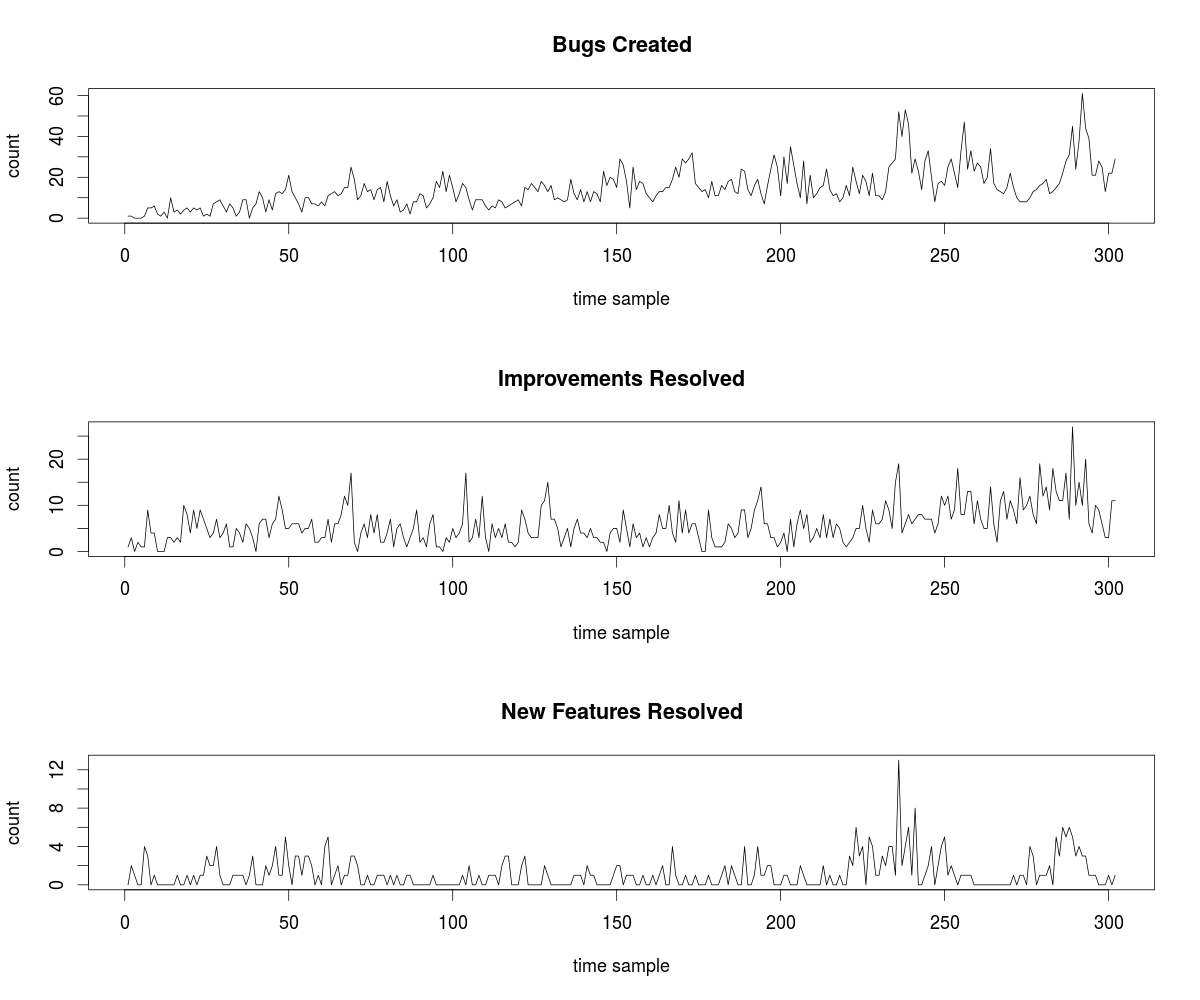
\includegraphics[width=\textwidth]{assets/time_series}
\caption{Time series data generated by sampling the MongoDB dataset with a 7-day sample period.}
\label{fig:time_series}
\end{center}
\end{figure}

\subsection*{Stationarity Testing}

Before modeling, the time series were all checked for stationarity. The result of the ADF unit root and KPSS stationarity tests are listed in tables \ref{tab:unit_root_results} and \ref{tab:stationarity_results}, respectively. Remember that for these tests, we need low significance for the unit root test and high significance for the stationarity test. This will allow us to reject the hypothesis that a time series has a unit root (is not stationary) and fail to reject the hypothesis that the time series is stationary. 

The unit root tests showed less than $1\%$ significance for all time series. However, the stationarity test also showed low significance. Since there is disagreement in the test results, the time series will all be differenced and the tests re-run.

\begin{table}[h!]
  \centering
  \begin{tabular}{ c | r r | r r | r r }
      & \multicolumn{2}{|c|}{$Y_{bug}$} & \multicolumn{2}{|c|}{$Y_{imp}$} & \multicolumn{2}{|c}{$Y_{new}$} \\
    Statistic & value & signif. & value & signif. & value & signif. \\
    \hline
    $\tau_2$ & -5.0203 & $< 1\%$ & -7.4022 & $< 1\%$ & -7.8448 & $< 1\%$ \\
    $\phi_1$ & 12.6505 & $< 1\%$ & 27.4154 & $< 1\%$ & 30.7709 & $< 1\%$ \\
    \hline
  \end{tabular}
\caption{Results of running the augmented Dickey-Fuller unit root test on $Y_{bug}$, $Y_{imp}$, and $Y_{new}$. The test is ran using an intercept-only regression model.}
\label{tab:unit_root_results}
\end{table}

\begin{table}[h!]
  \centering
  \begin{tabular}{ c | r r }
    Time series & statistic & signif. \\
    \hline
    $Y_{bug}$ & 2.8521 & $< 1\%$ \\
    $Y_{imp}$ & 2.0208 & $< 1\%$ \\
    $Y_{new}$ & 0.5269 & $2.5-5\%$ \\
    \hline
  \end{tabular}
\caption{Results of running the KPSS stationarity test on $Y_{bug}$, $Y_{imp}$, and $Y_{new}$. The test is ran assuming a constant-only deterministic component.}
\label{tab:stationarity_results}
\end{table}

After differencing we obtain the time series shown in figure \ref{fig:differenced_time_series}, which will be referred to as $Y_{\bigtriangledown bug}$, $Y_{\bigtriangledown imp}$, and $Y_{\bigtriangledown new}$. Now, the result of the unit root and stationarity test (listed in tables \ref{tab:first_diff_unit_root_results} and \ref{tab:first_diff_stationarity_results}) both agree. That is, we can reject the hypothesis that a unit root is present at the $1\%$  significance level and we have significance to accept stationarity with greater than $10\%$ significance. Hence, the differenced time series will be used to move forward with modeling.

\begin{figure}[htbp!]
\begin{center}
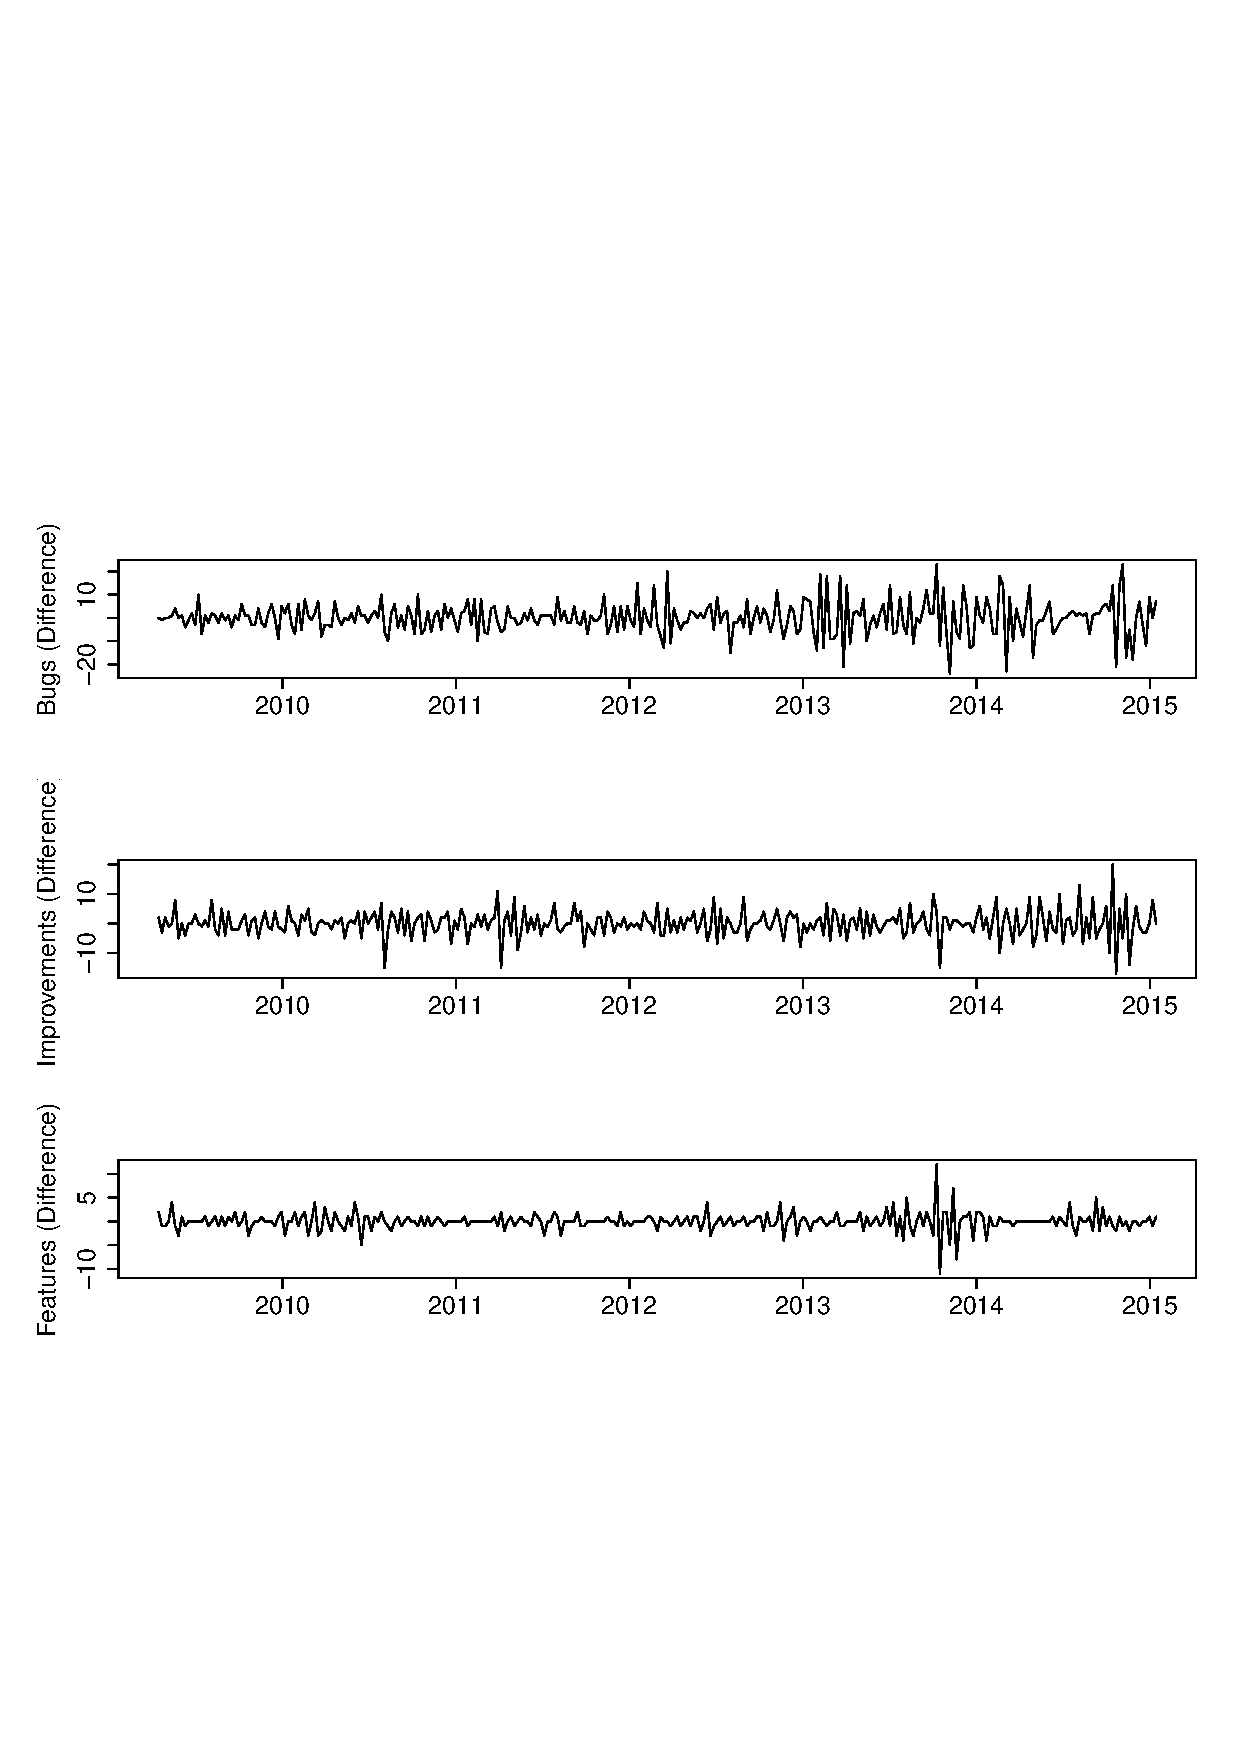
\includegraphics[width=\textwidth]{assets/time_series_diff}
\caption{Differenced time series data.}
\label{fig:differenced_time_series}
\end{center}
\end{figure}

\begin{table}[h!]
  \centering
  \begin{tabular}{ c | r r | r r | r r }
      & \multicolumn{2}{|c|}{$Y_{\bigtriangledown bug}$} & \multicolumn{2}{|c|}{$Y_{\bigtriangledown imp}$} & \multicolumn{2}{|c}{$Y_{\bigtriangledown new}$} \\
    Statistic & value & signif. & value & signif. & value & signif. \\
    \hline
    $\tau_2$ & -17.6529 & $< 1\%$ & -20.4382 & $< 1\%$ & -21.8989 & $< 1\%$ \\
    $\phi_1$ & 155.8144 & $< 1\%$ & 208.8647 & $< 1\%$ & 239.7814 & $< 1\%$ \\
    \hline
  \end{tabular}
\caption{Results of running the augmented Dickey-Fuller unit root test on the differenced time series}
\label{tab:first_diff_unit_root_results}
\end{table}

\begin{table}[h!]
  \centering
  \begin{tabular}{ c | r r }
    Time series & statistic & signif. \\
    \hline
    $Y_{\bigtriangledown bug}$ & 0.0115 & $> 10\%$ \\
    $Y_{\bigtriangledown imp}$ & 0.0127 & $> 10\%$ \\
    $Y_{\bigtriangledown new}$ & 0.0127 & $> 10\%$ \\
    \hline
  \end{tabular}
\caption{Results of running the KPSS stationarity test on the differenced time series}
\label{tab:first_diff_stationarity_results}
\end{table}

\subsection*{Time Windowing}
A 78-week time window (approximately 18 months) was established to restrict model scope. Three of these windowed periods, non-overlapping, were kept for modeling, and will be denoted $W_{1-78}$, $W_{79-156}$, and $W_{157-234}$.

\subsection*{Time Series Model}

The VARX model, discussed in the \nameref{sec:time_series_modeling} section, was used to model the time series. This model was used because there are multiple time series to be considered jointly. $Y_{\bigtriangledown new}$ and $Y_{\bigtriangledown imp}$ time series were both considered exogenous, so that hypothetical future values could be considered in comparison of release plans, as discussed in the \nameref{sec:motivation} section.

\subsection*{Model Specification \& Estimation}

By selecting $K_{min} = 4$, a maximum model order is obtained by
\begin{equation}
p_{max} = \left \lfloor \frac{78}{(3)(4)} \right \rfloor = \lfloor 6.5 \rfloor = 6
\end{equation}

Models of order $1,2,...,p_{max}$ were estimated for later diagnostic checking.

\subsection*{Model Diagnostic Checking}

Candidate models were tested for stability and inadequacy. A $5\%$ significance level was used in the Ljung-Box test. The results for each windowed period are shown in table \ref{tab:diagnostic_results}. All model orders were stable for all windowed periods. Several model orders were found to be inadequate by the Ljung-Box test: orders 1-2 for period $W_{1-78}$, and order 5 for period $W_{157-234}$.

\begin{table}[h!]
  \centering
  \begin{tabular}{ c | r r | r r | r r }
      & \multicolumn{2}{|c|}{$W_{1-78}$} & \multicolumn{2}{|c|}{$W_{79-156}$} & \multicolumn{2}{|c}{$W_{157-234}$} \\
    Model order & stable & p-value & stable & p-value & stable & p-value \\
    \hline
    1 & Yes & 0.009061 & Yes & 0.4478 & Yes & 0.09453 \\
    2 & Yes & 0.01401 & Yes & 0.5866 & Yes & 0.1255 \\
    3 & Yes & 0.2052 & Yes & 0.6470 & Yes & 0.1753 \\
    4 & Yes & 0.1288 & Yes & 0.7596 & Yes & 0.09363 \\ 
    5 & Yes & 0.3363 & Yes & 0.6133 & Yes & 0.04656 \\
    6 & Yes & 0.2818 & Yes & 0.3838 & Yes & 0.05703 \\
    \hline
  \end{tabular}
\caption{Results of running stability and Ljung-Box test on each windowed period.}
\label{tab:diagnostic_results}
\end{table}

\subsection*{Model Selection}
Models that were not rejected for instability or inadequacy were then compared and the best for each windowed period was selected by AIC selection criterion. The results of selection are shown in table \ref{tab:selection_results}, with orders 4, 1, and 1 being chosen for periods $W_{1-78}$, $W_{79-156}$, and $W_{157-234}$, respectively. The fit for each of these models is demonstrated by plotting one-step predictions along with actual values, shown for each model in figure \ref{fig:one_step_predictions}.

\begin{table}[h!]
  \centering
  \begin{tabular}{ c | r | r | r }
    ~ & \multicolumn{3}{|c}{AIC score} \\
    Model order & $W_{1-78}$ & $W_{79-156}$ & $W_{157-234}$ \\
    \hline
    1 & N/A & 429.8 & 477.9 \\
    2 & N/A & 439.3 & 482.4 \\
    3 & 400.8 & 440.9 & 489.7 \\
    4 & 400.3 & 450.2 & 499.9 \\ 
    5 & 404.0 & 456.7 & N/A \\
    6 & 414.9 & 461.7 & 508.8 \\
    \hline
  \end{tabular}
\caption{Results of model selection, using AIC score to compare models of different order.}
\label{tab:selection_results}
\end{table}

\begin{figure}
\centering
\subfloat[Windowed period $W_{1-78}$]{
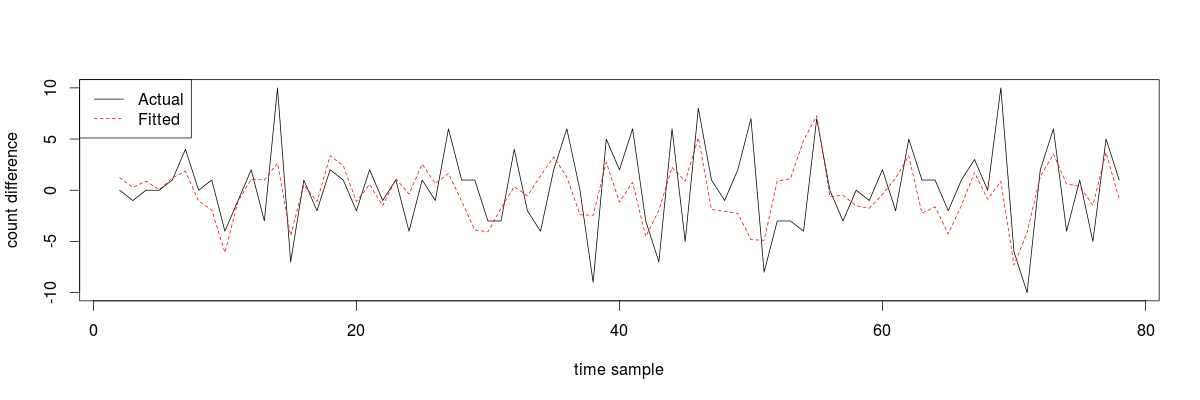
\includegraphics[width=\textwidth]{assets/1-78_one-step_predictions}
}\\
\subfloat[Windowed period $W_{79-156}$]{
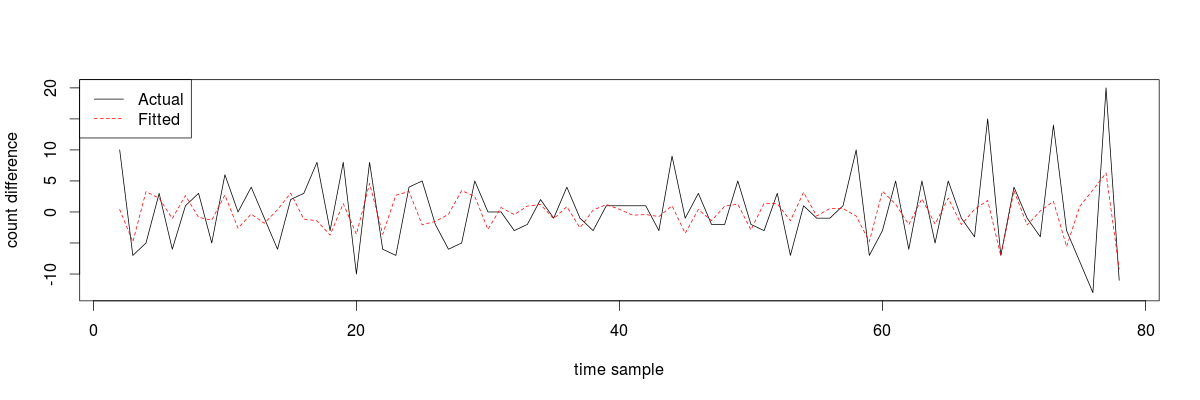
\includegraphics[width=\textwidth]{assets/79-156_one-step_predictions}
}\\
\subfloat[Windowed period $W_{157-234}$]{
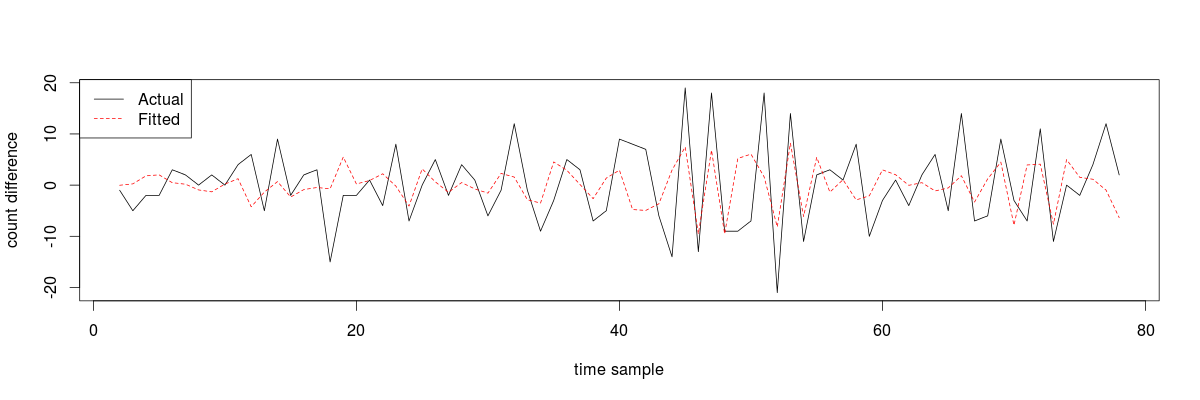
\includegraphics[width=\textwidth]{assets/157-234_one-step_predictions}
}%
\caption{One-step predictions vs actual values, for each model selected by AIC score.}
\label{fig:one_step_predictions}
\end{figure}


%\begin{figure}[htbp!]
%\begin{center}
%\includegraphics[width=\textwidth]{assets/one-step_predictions}
%\caption{Results of model fitting shown by one-step predictions.}
%\label{fig:one_step_predictions}
%\end{center}
%\end{figure}

\subsection*{Model Hypothetical scenarios}

TODO 
%Lastly, the effects of hypothetical future values of $Y_{new}$ and $Y_{imp}$ are considered. Such hypothetical future values would be considered in the context of a software release plan. Different plans can be compared by their predicted values of $Y_{bug}$. The result of one-step $Y_{bug}$ predictions for hypothetical $Y_{new}$ and $Y_{imp}$ values are shown in Figures \ref{fig:scenarios2d} and \ref{fig:scenarios3d}. We see that using the VARX model, the one-step prediction case results in a linear relationship between hypothetical exogenous values and the predicted endogenous value.
%
%\begin{figure}[htbp!]
%\begin{center}
%\includegraphics[width=\textwidth]{assets/scenarios2d}
%\caption{The effect of hypothetical future values for $Y_{new}$ and $Y_{imp}$, shown as a series of lines in 2D.}
%\label{fig:scenarios2d}
%\end{center}
%\end{figure}
%
%\begin{figure}[htbp!]
%\begin{center}
%\includegraphics[width=\textwidth]{assets/scenarios3d}
%\caption{The effect of hypothetical future values for $Y_{new}$ and $Y_{imp}$, shown as a plane in 3D.}
%\label{fig:scenarios3d}
%\end{center}
%\end{figure}

\section*{Proposed Work}
\label{sec:proposed_work}

After applying the data and modeling methodologies to the MongoDB dataset, a model is in-hand for each windowed time period. However, to adequately answer the question of whether such models can be used in release planning, further still remains. This proposed work is as follows:

\begin{enumerate}
\item
Apply the model to hypothetical \say{release plans}, that is, predict future values of $Y_{bug}$ using hypothetical future values of $Y_{imp}$ and $Y_{new}$. Keeping in mind the prediction confidence intervals, this would indicate how such a model might be in release-planning.

\item
Follow the same methodologies with two other SW projects.
\end{enumerate}

The time estimated to complete the proposed work is summarized in the timeline shown in table \ref{tab:timeline}.

\begin{table}[h]
\centering
\begin{tabular}{ p{2.5in} l l}
\hline
Task & Date \\
\hline
Form committee & Mar 9-13 \\
Present proposal & Mar 18 \\
Respond to committee feedback & Mar 18 - Apr 8 \\
Apply models for release planning & Apr 1-15 \\
Repeat on two other SW projects & Apr 15 - May 6 \\
\hline
\end{tabular}
\caption{Timeline for proposed work}
\label{tab:timeline}
\end{table}

%%\appendix
%%\section{Software Requirements}
%%\label{sw_reqs}
%%The software developed so far has been used for data collection and analysis. The scripts used can be run on any platform that supports Python and R. Besides this basic requirement, here are the other dependencies:
%%\paragraph{Python dependencies:}
%%\begin{itemize}
%%\item
%%docopt: for defining command-line interfaces and parsers. See the \href{https://github.com/docopt/docopt}{GitHub page} for installation instructions.
%%\item
%%BeatifulSoup: for processing XML files. See the \href{http://www.crummy.com/software/BeautifulSoup}{support page} for installation instructions.
%%\end{itemize}
%%
%%\paragraph{R dependencies:}
%%\begin{itemize}
%%%\item
%%%devtools: adds github\_install function. Install by running ``\verb|install.packages("devtools")|" on the R command line.
%%%\item{docopt: for defining command-line interfaces and parsers. See the \href{https://github.com/edwindj/docopt.R}{GitHub page} for installation instructions.}
%%\end{itemize}


\bibliography{references}
\bibliographystyle{abbrv}

\end{document}